% !TEX encoding = UTF-8 Unicode
\chapter{La \mt Causailté de Granger}
\label{chap5}

\section{Méthodologie}
\subsection{Le modèle  autorégressive - AR}
Dans les domaines de statistiques et du traitement du signal, le modèle autorégressive (AR) est une représentation d'un type de processus aléatoire. il est utilisé pour décrire certains processus  qui varies suivre le temps dans la nature, l'économie, etc. Dans ce modèle de régression, la variable de réponse dans la période de temps précédente est devenue le prédicteur et les erreurs ont nos hypothèses habituelles sur les erreurs dans un modèle de régression linéaire simple. L'ordre d'une autorégression est le nombre de valeurs immédiatement précédentes dans la série qui sont utilisées pour prédire la valeur à l'heure actuelle. 

La notation $AR(p)$ indique un modèle autorégressif avec l'ordre $p$, le modèle $AR(p)$ est définit comme : 
$$X_t = c + \sigma_{i = 1}^{p} \varphi_i  X_{t-1} + \varepsilon_t    $$
 où $\varphi_i, ..., \varphi_p$ sont les paramètre du  modèle, $c$ est un nombre constant, et $\varepsilon_t$ est le bruit blanc.
 
 Certaines contraintes de paramètres sont nécessaires pour que le modèle reste stationnaire. Par exemple, le processus du modèle $AR(1)$ avec $ | \varphi_1 | \geq 1 $ n'est pas stationnaire. Le processus AR le plus simple est $AR(0)$ qui n'a aucune dépendance entre les termes. Seul le terme erreur/ bruit contribue à la sortie du processus. 
 
 Pour un processus $AR(1)$ avec un $\varphi$ positif, seul le terme précédent dans le processus et le terme de bruit contribuent à la sortie. Si $\varphi$ est proche de 0, alors le processus ressemble toujours au bruit blanc, mais lorsque $\varphi$  s'approche de 1, la sortie obtient une grande contribution du terme précédent par rapport au bruit. Cela entraîne un lissage ou une intégration de la sortie, similaire à un filtre passe-bas. 
 
Pour un processus $AR(2)$, les deux termes précédents et le terme de bruit contribuent à la sortie. Si $\varphi_1$  et $\varphi_2$  sont tous deux positifs, la sortie ressemblera à un filtre passe-bas, la partie haute fréquence du bruit diminuant. Si $\varphi_1$ est positif alors que $\varphi_1$  est négatif, le processus favorise les changements de signe entre les termes du processus. La sortie oscille. Cela peut être assimilé à une détection de bord ou à une détection de changement de direction.

La performance prédictive du modèle autorégressive peut être évaluée dès que l’estimation a été effectuée si la validation croisée est utilisée. Alternativement, après un certain temps donc des paramètres sont estimés, davantage de données seront disponibles et les performances prédictives pourront être évaluées à l'aide des nouvelles données.
 
\subsection{Le modèle autoregressive vectorielle - VAR}
L’autorégression vectorielle (VAR) est un modèle de processus stochastique utilisé pour capturer les interdépendances linéaires entre plusieurs séries temporelles. Les modèles VAR généralisent le modèle autorégressif univarié (modèle AR) en permettant plusieurs variables évolutives. Toutes les variables d'un VAR entrent dans le modèle de la même manière: chaque variable a une équation expliquant son évolution basée sur ses propres valeurs décalées, les valeurs décalées des autres variables du modèle et un terme d'erreur.La modélisation VAR ne nécessite pas autant de connaissances sur les forces influençant une variable que les modèles structurels à équations simultanées: la seule connaissance préalable requise est une liste de variables qui peuvent être supposées s’affecter intertemporellement. 

Le modèle VAR décrit l'évolution d'un ensemble de $k$ variable sur le même période d'échantillonnage $(t = 1,..., T)$ en tant que fonction linéaire de leur seules valeurs passées.  Les variables sont collectées dans des vecteur $y_t$ où $y_{i,t}$ est élément $i^{ième}$ au temps  observé $t$. Un modèle VAR d'ordre $p$, noté VAR(p) est définit par : 

$$y_t = c + A_{1}y_{t-1} + A_{2}y_{t-2} + \cdots + A_{p}y_{t-p} + e_t $$

où les arrière observation des i-période $y_{t-i}$ s'appelle le $i^{ième}$ retard de $y$, $c$ est un vecteur $k x 1$ de constance, $A_i$ est une matrice $k x k$ invariance dans le temps et $e_t$ est un vecteur $k x 1$ de terme d'erreur.

Le modèle VAR combine l'avantage du modèle autoregressive (AR) et des équations simultanées (SE)  en utilisant  la méthode minimisé les résidus et l'estimation de plusieurs variables dans un même système. De même, il surmonte l'inconvénient des SE qu'il ne se soucie pas de l'endogénéité des variable économiques. Les variables macroéconomiques sont souvent endogènes lorsqu'elles interagissent les unes avec les autres. Cet attribut rend la méthode de régression multiple utilisant une équation de régression multiple lors de la déviation de l'estimation. Ce sont les raisons fondamentales qui rendent le modèle VAR si populaires dans la recherche macroéconomique.

\subsection{La méthode causalité de Granger}
Le test de causalité de Granger (CA) est un test d'hypothèse statistique permettant de déterminer si une série temporelle est utile en prévoir une autre série temporelle, proposé pour la première fois en 1969 \cite{granger1969}. Cette méthode est reconnu comme le principal progrès sur le problème de causalité. L'idée principal de la méthode CA est : $Y_t$ cause $X_t$ si l’on est mieux capable de prédire $X_t$ à partir de l’ensemble des informations disponibles qu’à partir de ce même ensemble privé de $Y_t$\cite{granger1969,granger1980}. Si cette condition est satisfaite, cela signifie que $Y_t$ contient des informations exclusive qui ne sont pas présentes dans toutes les autres séries temporelles et que cette information est utile pour prédire la série temporelle $X_t$ d'intérêt. 

La causalité de Granger est basée sur deux principes : 
\begin{itemize} 
\item[$\bullet$] La cause se produit avant son effet;
\item[$\bullet$] La cause produit des changements uniques dans l'effet. En d'autres termes, la série temporelle causale contient des informations uniques sur la série temporelle d'effet qui ne sont pas disponibles autrement.
\end{itemize} 
Soit $I(t)$ l'ensemble des informations contenant toutes les informations pertinentes dans l'univers disponibles jusqu'à l'instant $t$ et $I_{-X}(t)$ est l'ensemble des informations de l'univers à l'exclusion de $X$ jusqu'au moment $t$. Donnant deux séries temporelles $X$ et $Y$, Granger a proposé de tester l'hypothèse suivante pour l'identification d'un effet causal de $X$ sur $Y$ :
 $$ \mathbb{P}[Y(t + 1) \in A \arrowvert I(t)] \neq \mathbb{P}[Y(t + 1) \in A \arrowvert I_{-X}(t)] $$
 
où $\mathbb{P}$ dénote une probabilité et $A$ est un ensemble arbitraire non vide. Si nous pouvons prouver l'hypothèse ci-dessus ou si nous pouvons rejeter l'hypothèse nulle :

 $$  \mathbb{P} [Y(t + 1) \in A \arrowvert I(t)] = \mathbb {P} [Y (t + 1) \in A \arrowvert I_{-X} (t)] ]$$  
 
 nous disons que $X$ Granger-cause $Y$.
 
 Plus précisément, considérons deux séries chronologiques stationnaires $ X_1 $ et $ X_2 $ avec un modèle autorégressif linéaire:
\begin{equation}
\begin{array}{c}
 X_1(t) = \sum\limits_{j = 1}\limits^pA_{11j}X_1(t-j) + \sum\limits_{j = 1}\limits^pA_{12j}X_2(t-j) + E_1(t)\\
 X_2(t) = \sum\limits_{j = 1}\limits^pA_{21j}X_1(t-j) + \sum\limits_{j = 1}\limits^pA_{22j}X_2(t-j) + E_2(t)
\end{array}
\end{equation}
 où $p$ est le nombre maximum d'observations retardées incluses dans le modèle, $A$ est la matrice contenant les coefficients du modèle (par exemple les contributions de chaque observation retardée) des valeurs prédites de $X_1(t) $ et $X_2(t)$. $E_1$ et $E_2$ sont des erreurs de prédictions pour chaque série temporelle. Si l'écart de $E_1$ (ou $E_2$) est réduit par l'inclusion de $X_2$ (ou $X_1$), alors il est dit que $X_2$ (ou $X_1$) Granger-cause $X_1$ (ou $X_2$). En d'autres termes, $X_2$ Granger-cause $X_1$ si le coefficient $A_ {12}$ est significativement différent de zéro. Cela peut être testé en effectuant un F-test de l'hypothèse nulle que $A_{12} = 0$, étant donné l'hypothèse de la stationnarité de la covariance sur $X_1 (t)$ et $X_2(t)$. L'ampleur d'une interaction Granger-causalité peut être estimée par le logarithme correspondante du F-statistique \cite{geweke1982}.
 
Le cadre de causalité de Granger peut être étendu pour résoudre le problème multivariable: étant donné les séries de temps $ p $, $ X_1 $, $ X_2 $, ..., $ X_ {p-1} $, $ X_p $, nous sommes intéressés à identifier quelle série temporelle Granger cause $X_i$. Il y a deux façons de résoudre ce problème:
\begin{itemize} 
\item[$\bullet$] Examiner les relations par paires dans chaque paire de séries temporelles;
\item[$\bullet$] Effectuer une autorégression vectorielle (VAR modèle) comme:
 \begin{equation}
 X_i(t) = \sum\limits_{j = 1}\limits^pA_{i, j}^TX_j^{t, lagged} + E
\end{equation}
 où $X_j^{t, lagged} = [X_j (t - L), ..., X_j (t - 1)] $ est la série temporelle retardée et $A_ {i, j}$ est le vecteur de coefficient. Ensuite, nous testons si $A_ {i, j}$ sont significativement différents de zéro. Une série temporelle $ {\displaystyle X_{i}} $ est appelée cause Granger d'une autre série temporelle $ {\displaystyle X_{j}} $ si au moins un des éléments $ {\displaystyle A_{L} (i, j)} $ pour $ {L = 1, \ldots, p} $ est significativement plus grand que zéro.
\end{itemize} 

Nous avons appliqué la causalité de Granger pour analyser la relation entre l'incidence de la DHF et les variables climatiques dans chacune des 64 provinces du Vietnam. Le test de causalité de Granger a été effectué en utilisant le package R \texttt{vars}  \cite{pfaff2013package}. Chaque provinces a été associée à là station climatique la plus proche de son centre de population comme la façon de celui de la méthode d'analyse ondelette au chapitre 4. Dans le premier test, nous avons effectué un test de causalité de Granger pour déterminer l'influence indépendance des facteurs climatiques sur l'incidence de la dengue dans chaque provinces au Vietnam. Puis, nous avons testé l'influence d'ensemble des facteur climatiques sur l'incidence de la dengue sur des provinces au Vietnam. Enfin, nous avons divisé la période en sub-séquence et nous testons la méthode GCA sur ces sub-séquence pour trouver la tendance d'influence des facteurs climatiques avec l'incidence de la dengue. 

\section{\Rs}

\subsection{\Rs d'analyse univariable}
Nous avons d'abord analysé la relation entre chaque facteur climatique et l'incidence de la dengue pour chaque province du Vietnam. Pour chaque province, nous avons appliqué la méthode GC et testé l'hypothèse nulle que le facteur climatique n'est pas la cause d'épidémiologie de la dengue. La figure \ref{Pic5_1} montre le résultat expérimentale de la méthode GCA sur notre données. Le vert indique les provinces pour lesquelles le test est significatif au niveau de $ \ alpha = 0,05 $, le gris indique les provinces pour lesquelles le test n'est pas significatif et le blanc indique les provinces pour lesquelles le test n'a pu être effectué faute de données. On a calculé le nombre total des provinces qui avaient la relation entre DHF et chacun des facteurs climatiques et leurs représente dans le tableau\ref{table1}.

\begin{table}[h]
\centering
\begin{tabular} { | c | c | c | c | c | c | c | c |}
\hline
Climatic factor & ta & tx & tm & rf & rh & sh & ah \\
\hline
Number of provinces & 33 & 34 & 34 & 13 & 12 & 10 & 39 \\
\hline
Percentage & 51.56 & 53.13 & 53.13 & 20.31 & 18.75 & 15.63 & 60.94 \\
\hline
\end{tabular}
\caption{Le nombre des provinces qui ont la relation entre le DHF et chacun des facteurs climatiques.} 
\label{table1}
\end{table}

Les résultats de la figure \ref{Pic5_1}  et le tableau \ref{table1} suggèrent que : 

\begin{itemize} 
\item[$\bullet$] la température et l'humidité absolue fortement influence l'incidence de la dengue, principalement dans les régions du centre et du sud du pays;
\item[$\bullet$] la pluviosité et l'humidité relative ont un impact faible sur l'incidence de la dengue dans certaines provinces;
\item[$\bullet$] les heures d'ensoleillement ont un impact important sur l'influence de la zone centrale.
\end{itemize} 


\begin{figure}[h]
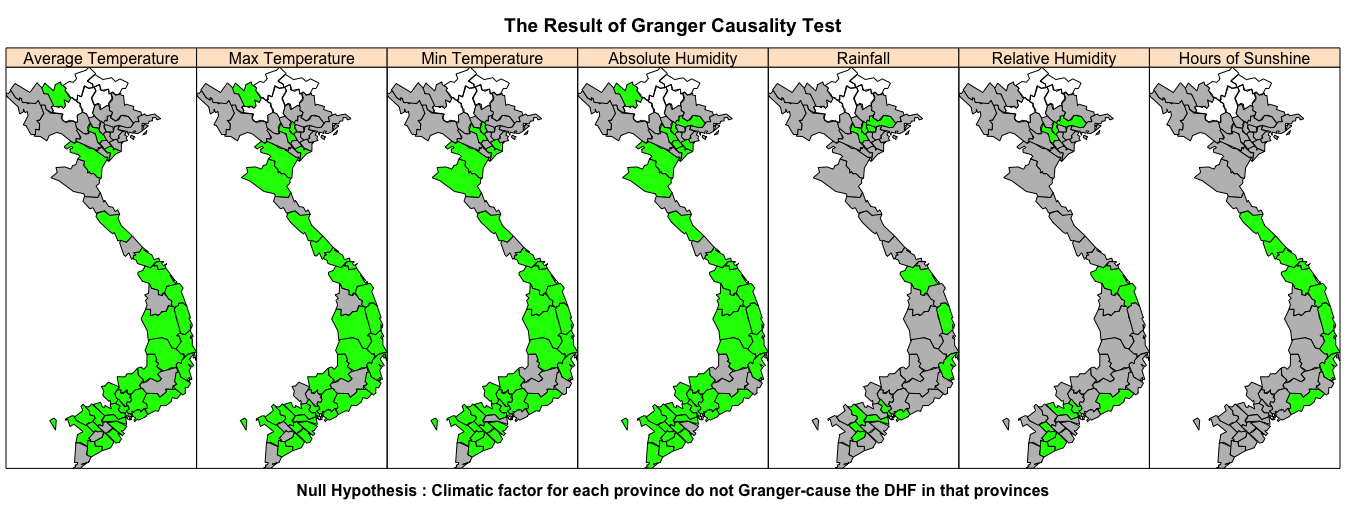
\includegraphics[width = \linewidth]{../figures/chap5/Pic5_1.png}
\caption{Résultats du test de causalité Granger pour chaque variable climatique et chaque province.}
\label{Pic5_1}	
\end{figure}

\subsection{\Rs d'analyse multivariable}
Dans cette étude, nous utilisons le GC multivariable pour analyser la relation entre DHF et l'impact de l'ensemble des facteurs climatiques au même moment. Nous avons combiné des paires de variable pour appliquer la méthode GCA multivariable. Cependant, parmi les trois variable de température : température moyenne (TA), température maximal (TX), température minimal (TM), nous choisissons uniquement la température moyenne pour combiner avec les autres variables. Pour chaque cas de test, nous avons compté le nombre des provinces qui avaient la relation entre DHF et chacun des paires des facteurs climatiques et leurs représente dans le tableau \ref{table2}. 

\begin{table}[h]
\begin{tabular} { | p{1.9cm} |  p{0.9cm} | p{0.9cm} | p{0.9cm} | p{0.9cm} | p{0.9cm} | p{0.9cm} | p{0.9cm} | p{0.9cm} | p{0.9cm} | p{0.9cm} | p{0.9cm} |}
\hline
Set of climatic factors & ta + rf & ta + rh & ta + sh & ta + ah & rf + rh & rf + sh & rf + ah & rh + sh & rh + ah & sh + ah \\
\hline
Number of provinces & 33 & 31 & 29 & 35 & 13 & 20 & 34 & 18 & 33 & 33 \\
\hline
Percentage & 51.56 & 48.44 & 45.31 & 54.69 & 20.31 & 31.25 & 53.13 & 28.13 & 51.56 & 51.56 \\
\hline
\end{tabular}
\caption{Le nombre de provinces a été conclu qui était la relation entre DHF et l'ensemble des paires des facteur climatique} 
\label{table2}
\end{table}

Nous pouvons voir clairement que les variables température et humidité absolue ont une grande influence sur la situation de DHF, que ce soit avec une analyse indépendant ou multivariée. Ce qui nous a surpris, c'est la combinaison entre les heures d'ensoleillement et les précipitations, les heures d'ensoleillement et l'humidité relative nous donnent un meilleur résultat qu'une analyse indépendante. Cela peut certainement arriver parce que les heures d'ensoleillement et les précipitations sont négativement corrélées.
 
\subsection{\Rs d'analyse sous-séquence}

Dans cette analyse, nous effectuons une analyse sous-séquence  avec la méthode  GCA dans les deux cas univariable et multivariable pour analyser le développement des corrélation  d'épidémie et les facteurs climatiques sur des périodes de temps. À partir de janvier 1998, nous avons effectué l’analyse sur une période de 6, 7, 8 et 9 ans au lieu de 12 ans. Ensuite, nous répétons le processus avec le temps de début de 3 mois plus tard que le test précédent. La figure \ref{fig_uni6} montre que les résultats de l'analyse de sous-séquence avec la longueur de la période sont égaux à 6 ans. Chaque point de l'axe abscisse représente une période d'analyse de six ans et l'axe ordonnée indique le nombre de villes dont on a conclu qu'elles étaient liées à la dengue et aux facteurs climatiques correspondants. Les figures \ref{fig_uni7}, \ref{fig_uni8}, \ref{fig_uni9} montrent le résultat de la sous-séquence univariable avec la longueur de la période égale à 7, 8 et 9 ans. Nous pouvons voir que l'influence des facteurs climatiques sur la DHF a tendance à augmenter avec le temps. Cela se reflète dans la valeur de croissance sur l'axe ordonnée de la plupart des variables météorologiques, où l'augmentation de la pluviométrie variable et de l'humidité absolue est la plus évidente. 

Les figures \ref{fig_multi6}, \ref{fig_multi7}, \ref{fig_multi8}, \ref{fig_multi9} représentent le résultat des tests de sous-séquence multivariable dans ces périodes. Nous constatons que la température et l’humidité absolue ont toujours des effets importants sur l’incident de la dengue lorsque leur combinaison avec d’autres variables augmente fortement avec le temps. De plus, la combinaison des précipitations et des heures d'ensoleillement, des précipitations et de l'humidité relative montre également leur effet latent lorsqu'elles sont combinées.

\begin{figure}[h]
\begin{center}
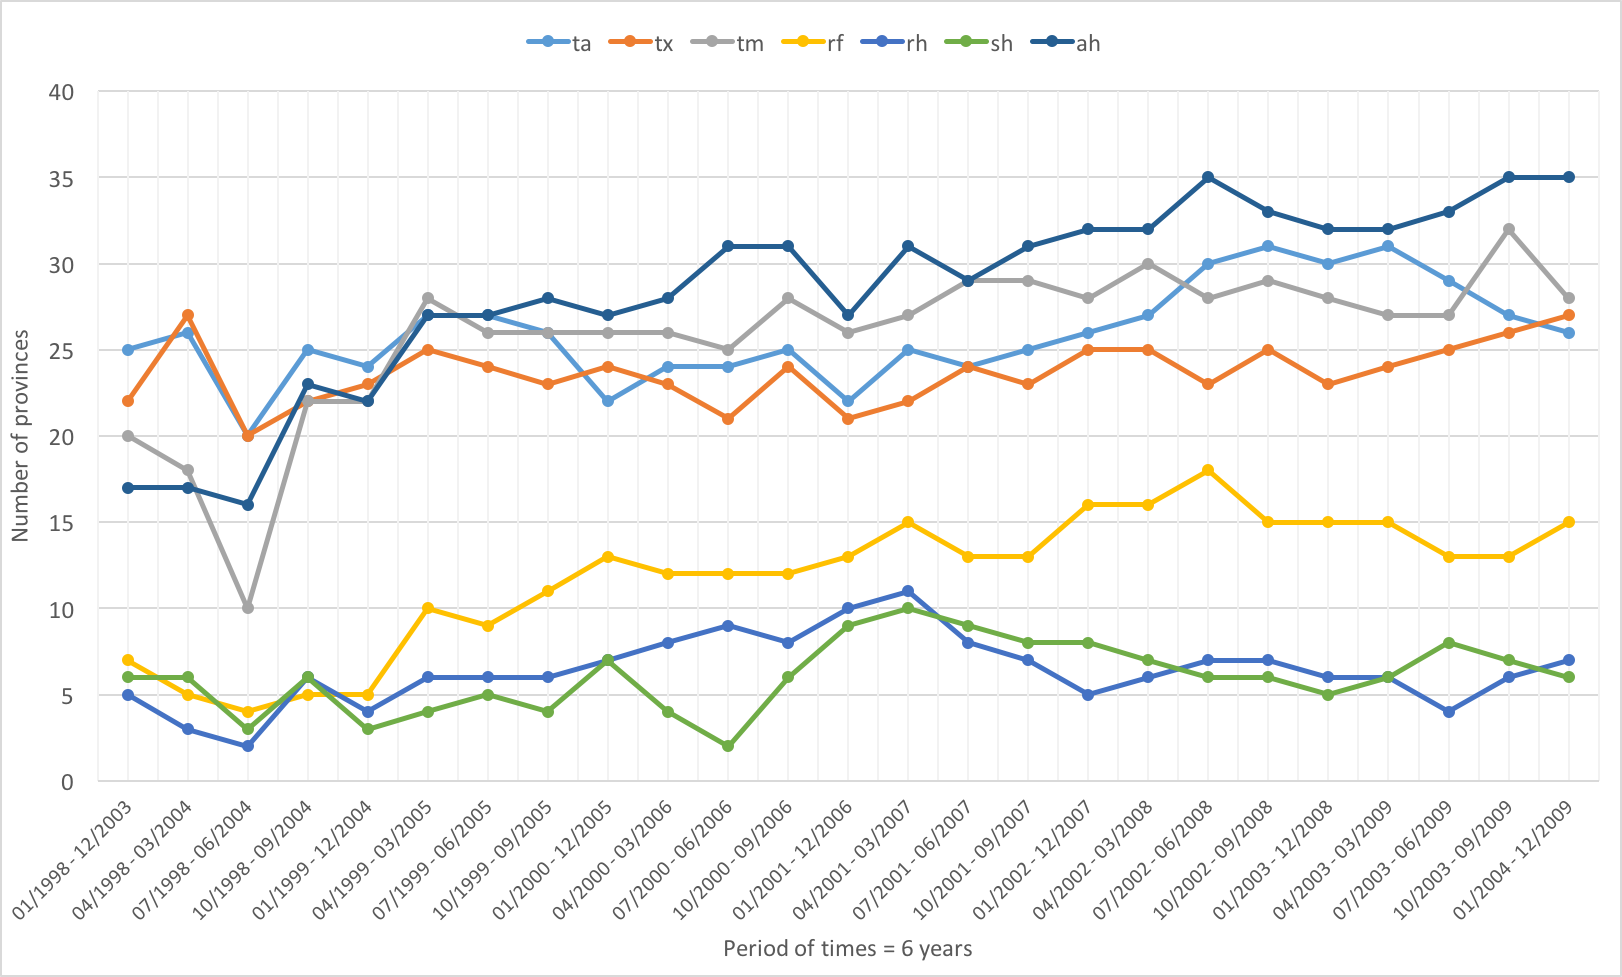
\includegraphics[width = \linewidth]{../figures/chap5/uni_6.png}
\caption{Le résultat du test sous-séquence avec la méthode GCA univariée. La durée de chaque période L = 6 ans }
\label{fig_uni6}	
\end{center}
\end{figure}


\begin{figure}[h]
\begin{center}
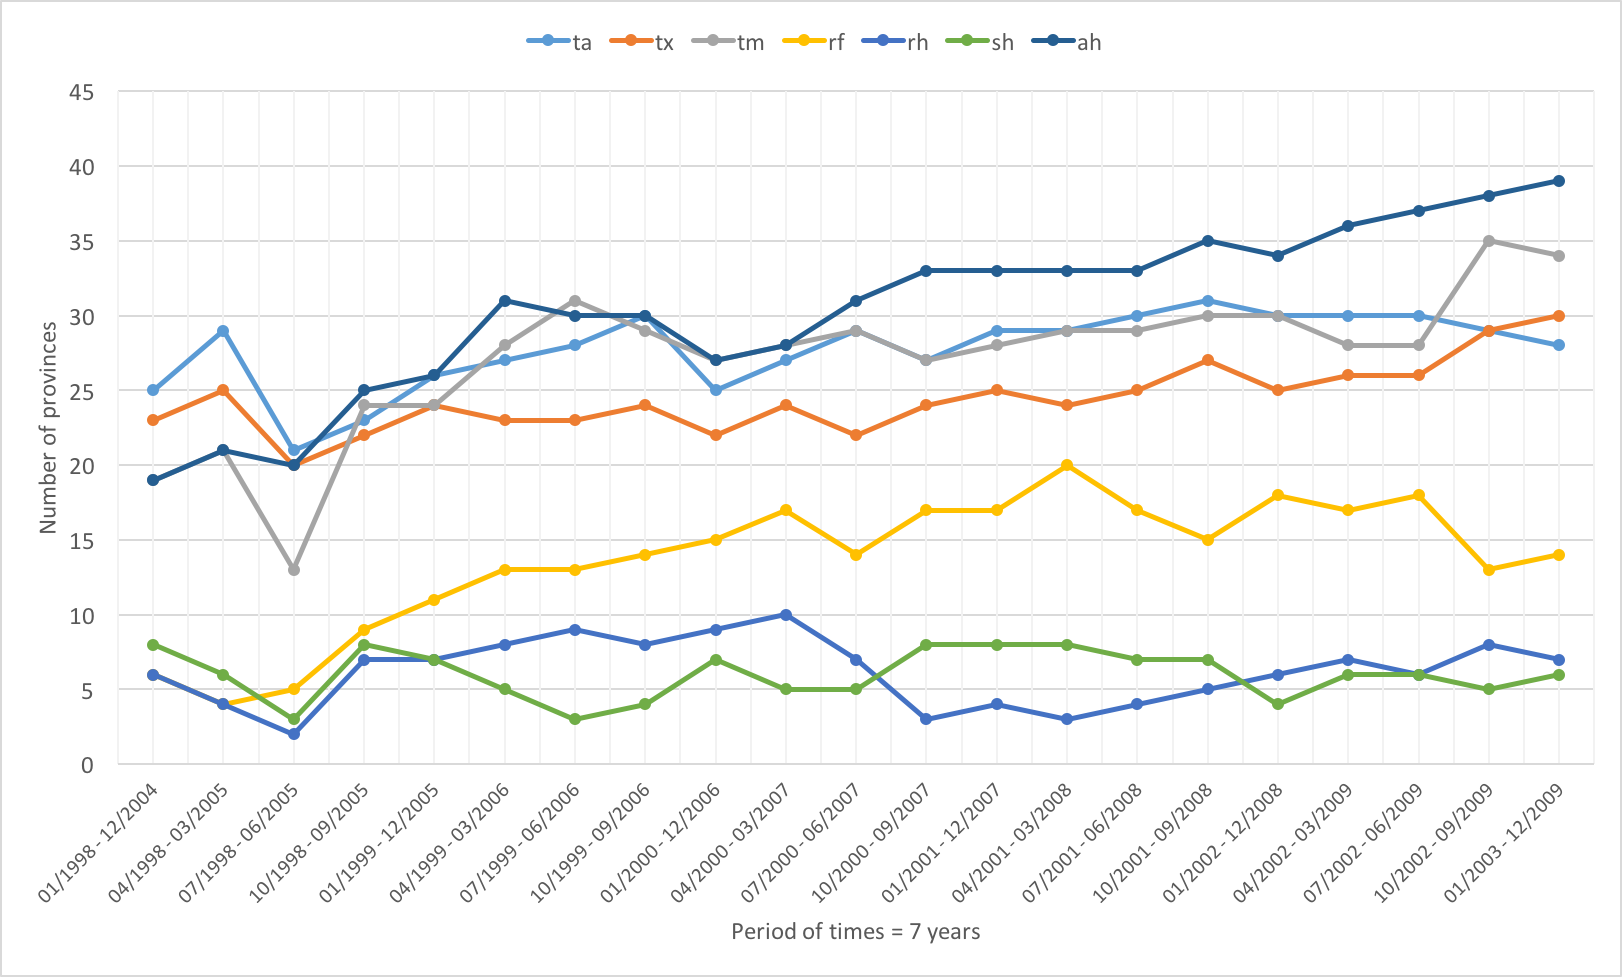
\includegraphics[width = \linewidth]{../figures/chap5/uni_7.png}
\caption{Le résultat du test sous-séquence avec la méthode GCA univariée. La durée de chaque période L = 7 ans }
\label{fig_uni7}	
\end{center}
\end{figure}

\begin{figure}[h]
\begin{center}
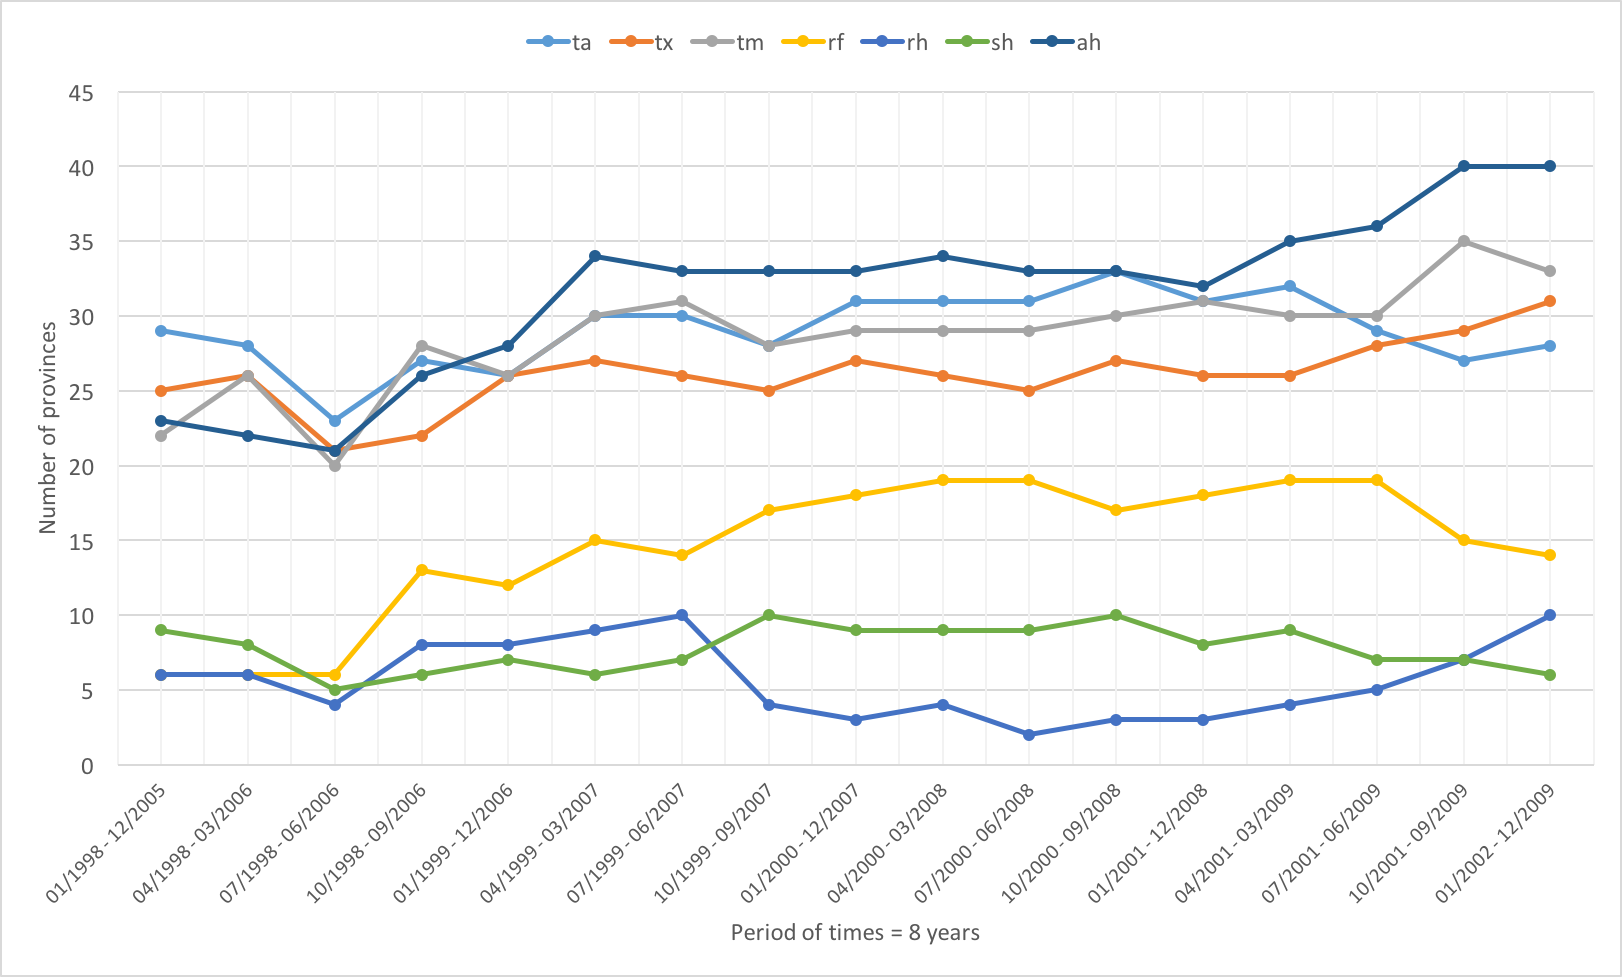
\includegraphics[width = \linewidth]{../figures/chap5/uni_8.png}
\caption{Le résultat du test sous-séquence avec la méthode GCA univariée. La durée de chaque période L = 8 ans }
\label{fig_uni8}	
\end{center}
\end{figure}

\begin{figure}[h]
\begin{center}
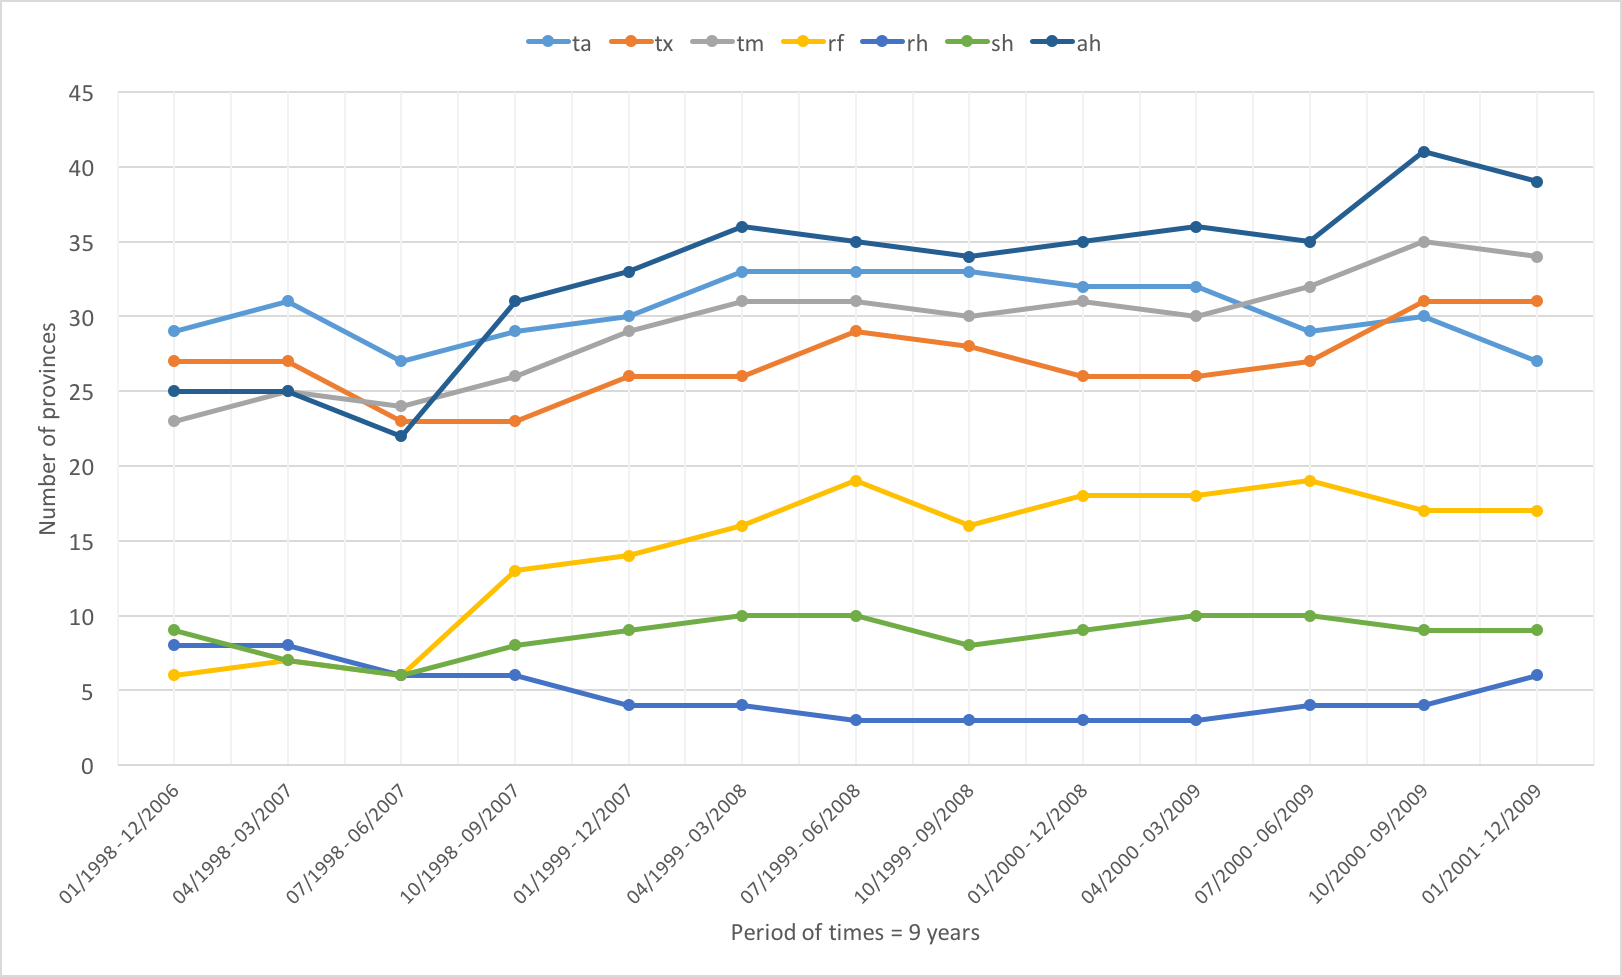
\includegraphics[width = \linewidth]{../figures/chap5/uni_9.png}
\caption{Le résultat du test sous-séquence avec la méthode GCA univariée. La durée de chaque période L = 8 ans }
\label{fig_uni9}	
\end{center}
\end{figure}


%% figure of multivariable subsequence test

\begin{figure}[h]
\begin{center}
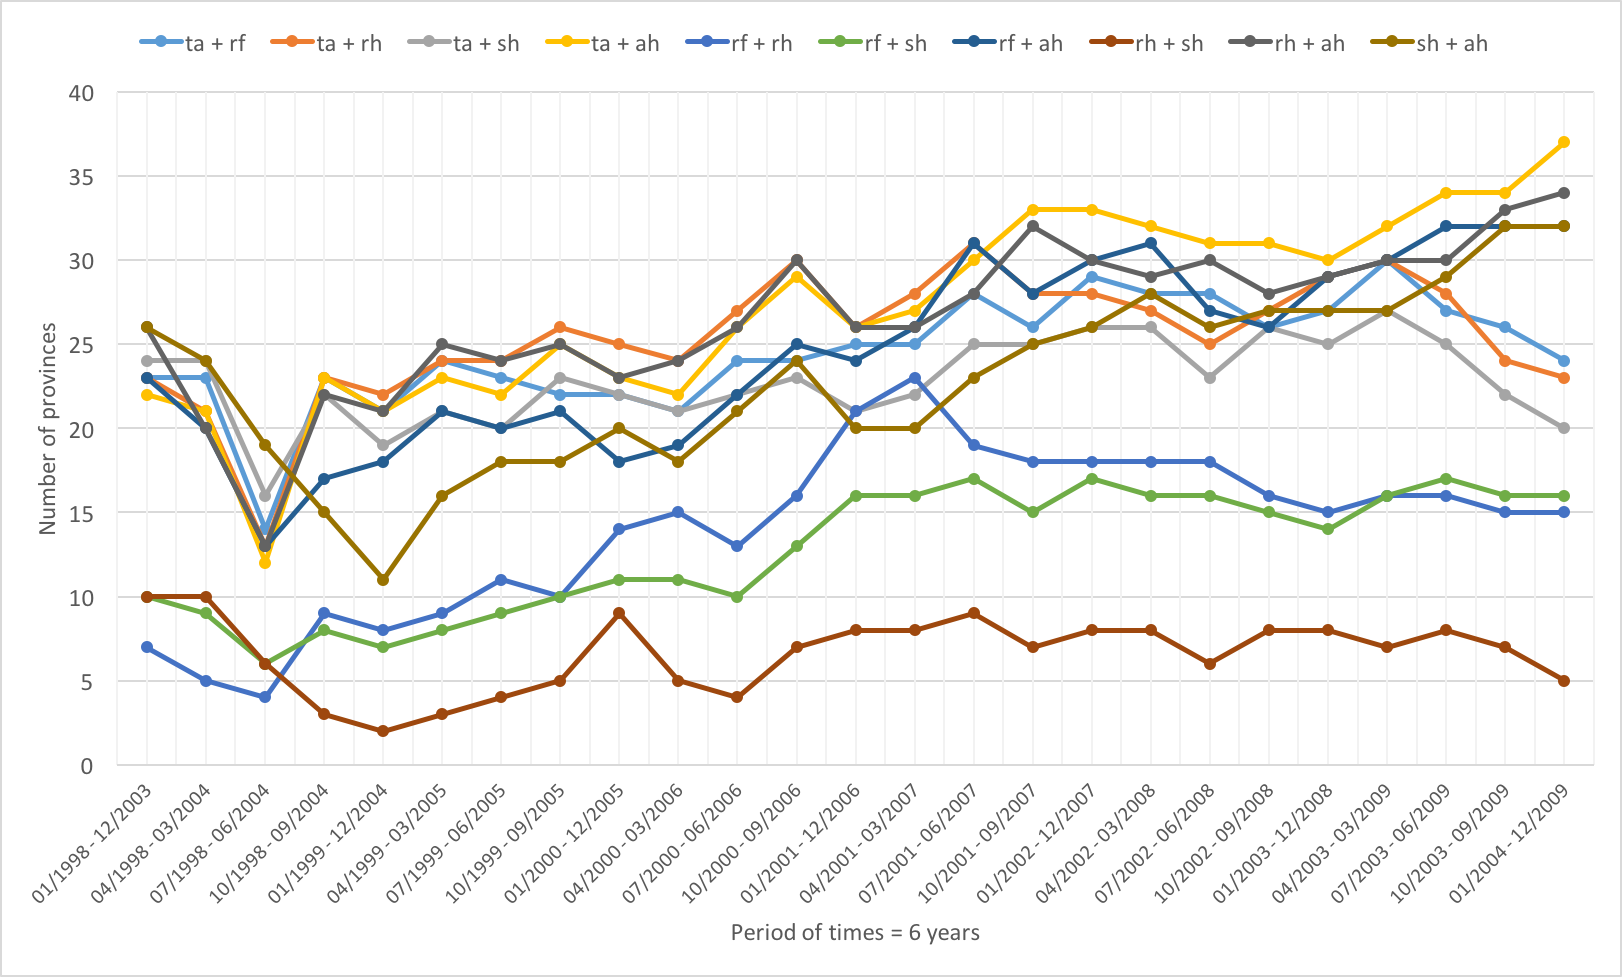
\includegraphics[width = \linewidth]{../figures/chap5/multi_6.png}
\caption{Le résultat du test sous-séquence avec la méthode GCA multivariée. La durée de chaque période L = 6 ans }
\label{fig_multi6}	
\end{center}
\end{figure}

\begin{figure}[h]
\begin{center}
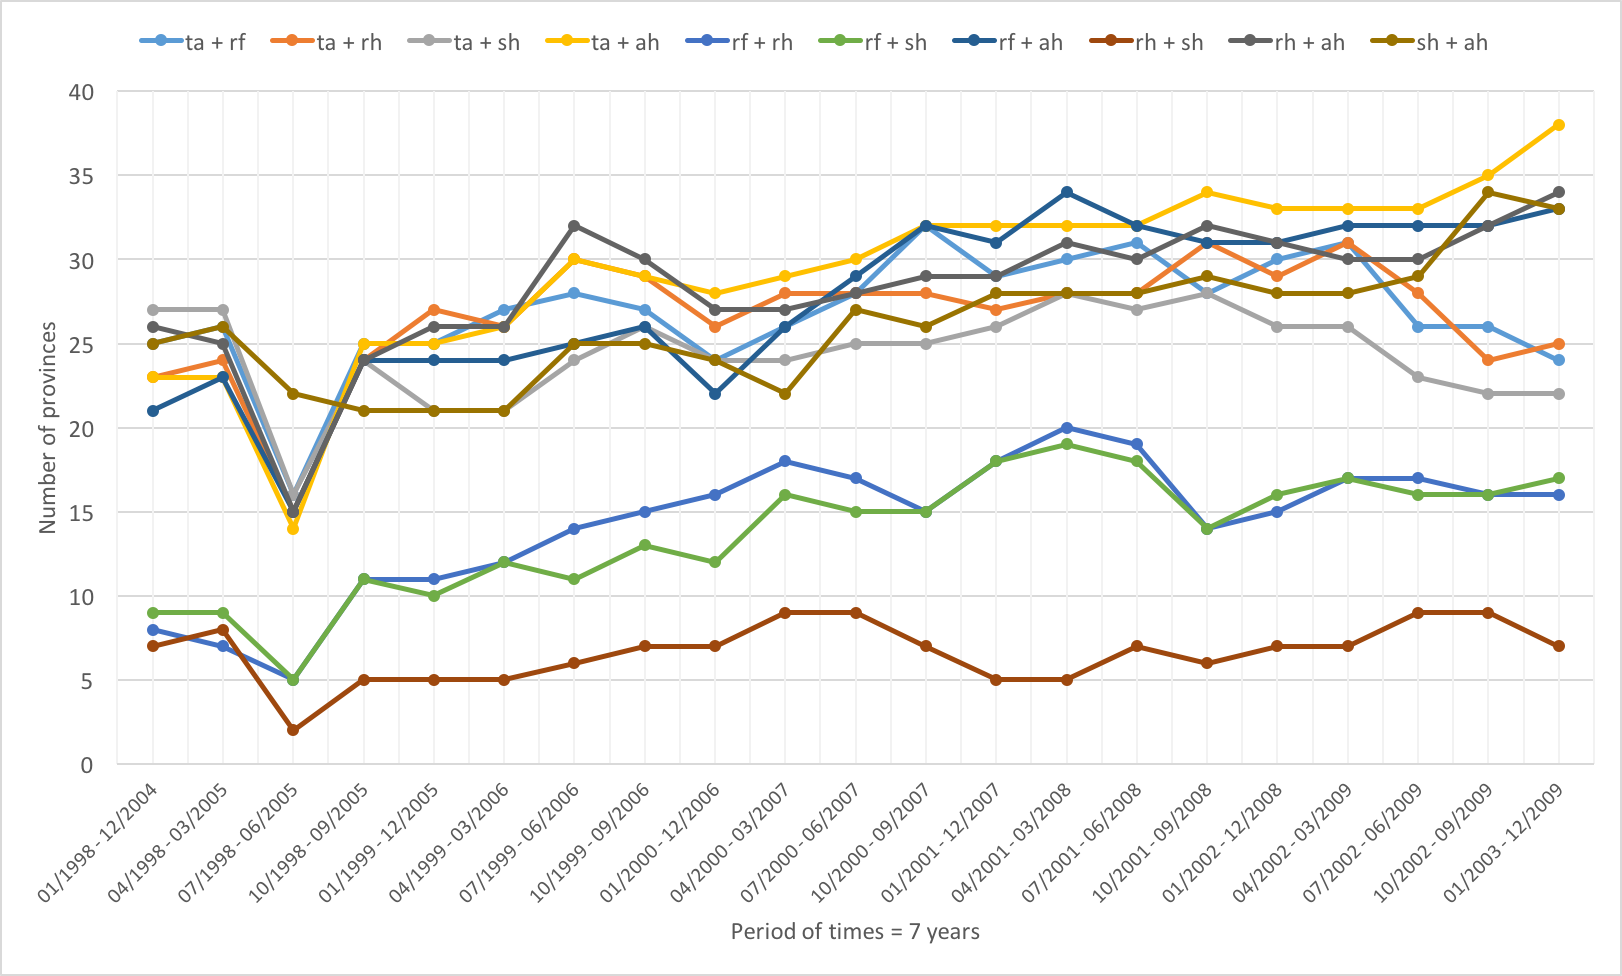
\includegraphics[width = \linewidth]{../figures/chap5/multi_7.png}
\caption{Le résultat du test sous-séquence avec la méthode GCA multivariée. La durée de chaque période L = 7 ans }
\label{fig_multi7}	
\end{center}
\end{figure}

\begin{figure}[h]
\begin{center}
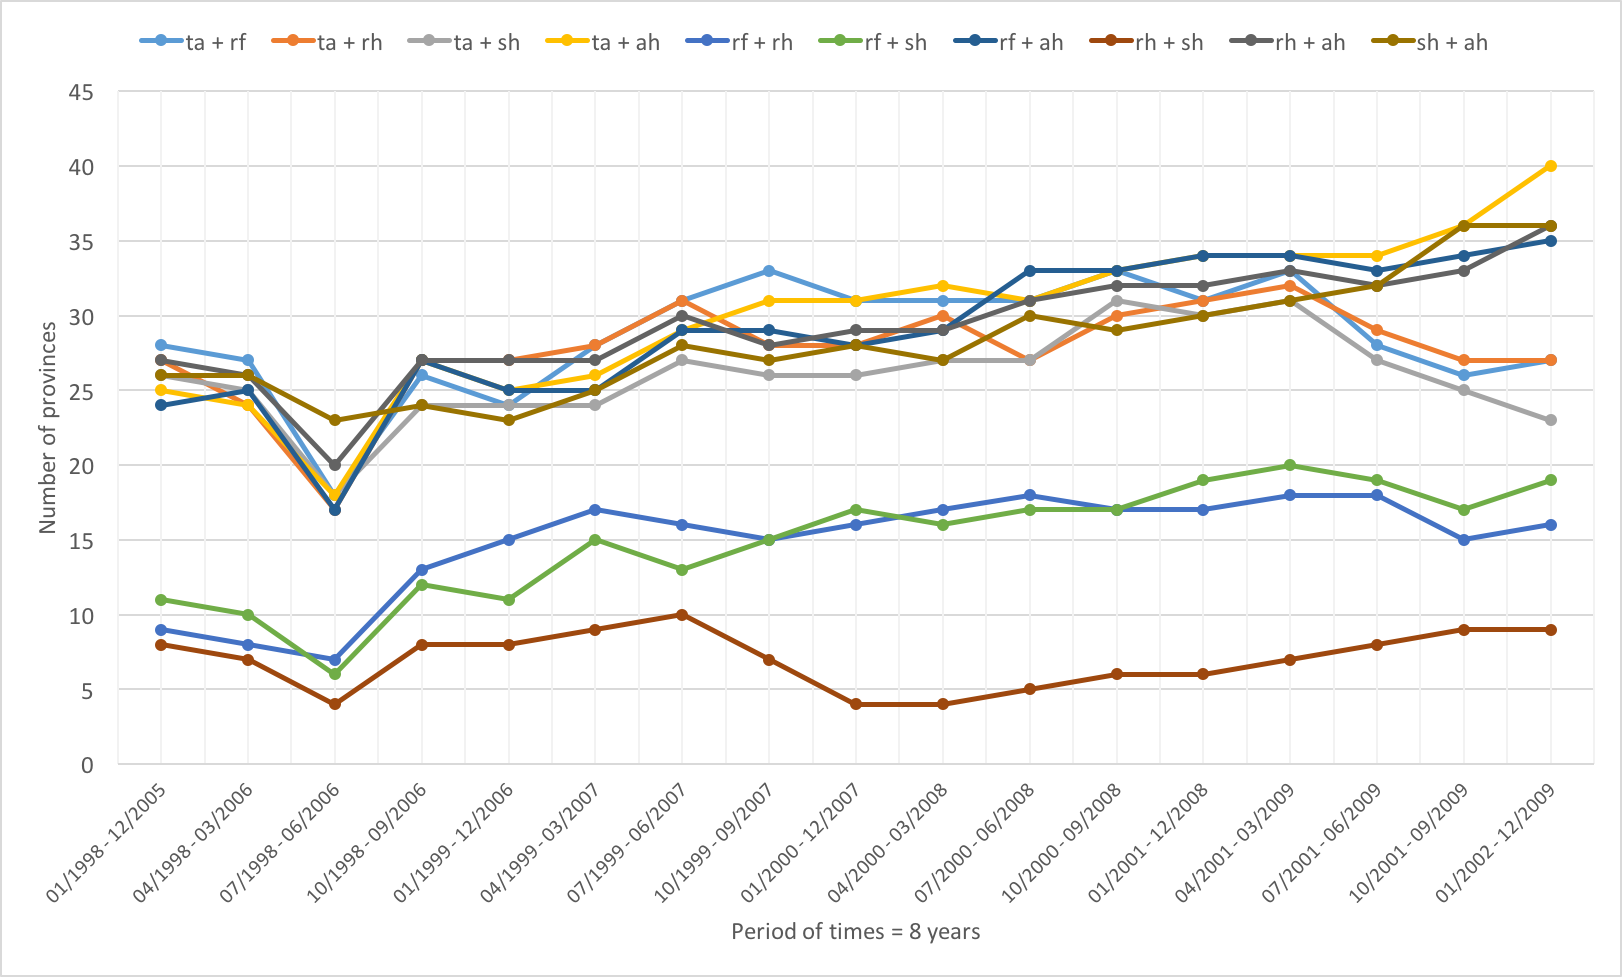
\includegraphics[width = \linewidth]{../figures/chap5/multi_8.png}
\caption{Le résultat du test sous-séquence avec la méthode GCA multivariée. La durée de chaque période L = 8 ans }
\label{fig_multi8}	
\end{center}
\end{figure}

\begin{figure}[h]
\begin{center}
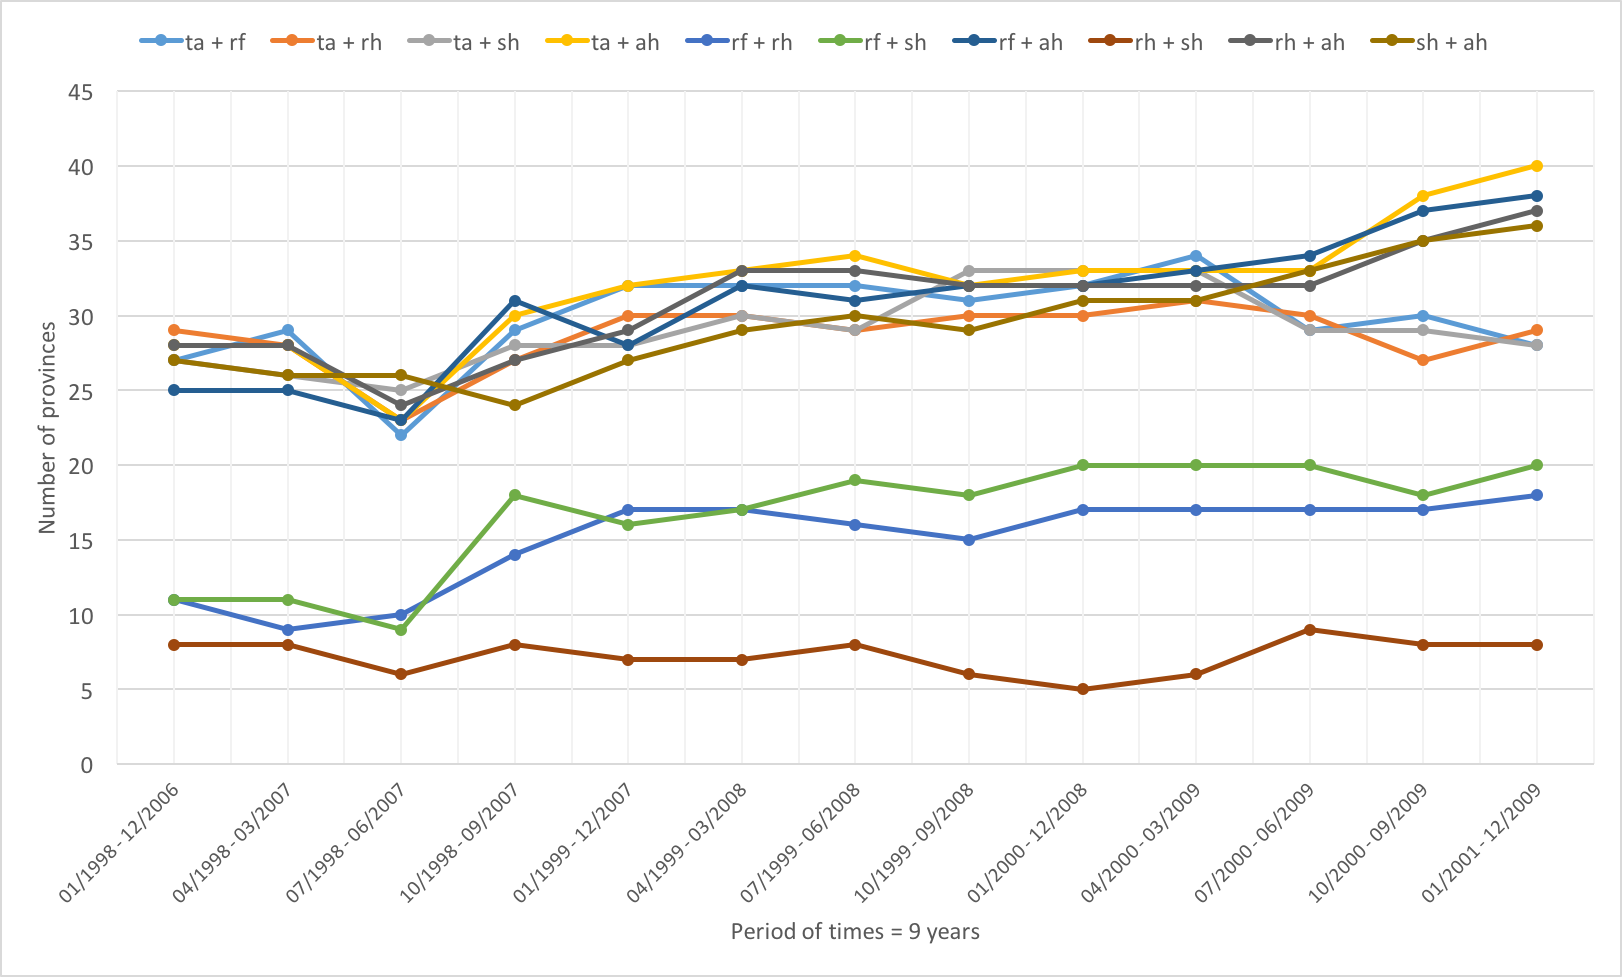
\includegraphics[width = \linewidth]{../figures/chap5/multi_9.png}
\caption{Le résultat du test sous-séquence avec la méthode GCA multivariée. La durée de chaque période L = 9 ans }
\label{fig_multi9}	
\end{center}
\end{figure}


Dans cette chapitre, nous avons appliqué la méthode GCA dans les deux cas univariable  et multivariable. Les résultats du test univariable montre que le température et l'absolue humidité est fortement influence l'incidence de la dengue dans les provinces du Vietnam. La pluviosité, l'humidité relative et l'heure du soleil ont des faible influence sur certains provinces du Vietnam. Cependant, dans les multivariable, l'humidité relative, la pluviosité et l'heure de soleil a montré des latent corrélations lorsque leurs combinaisons avait eu les nombre de provinces significatif plus grandes que ceux du test univariable. De plus, nous avons lancé les test de sous-séquence en appliquant la méthode GCA univariable et multivariable avec les différents périodes. Leurs résultats montre que les effets des facteurs environnementaux sur l'incidence de la dengue a augmenté avec le temps durant le période 1998 - 2010\ref{hoang2016}. Dans la chapitre après, nous utilisons une autre méthode pour recalculer l'effet des facteurs climatique sur l'incidence de la dengue pour affirmer les relations entres les facteurs environnementaux et l'influence de l'épidémie de la dengue.






